
\documentclass[twoside,12pt,a4paper]{report}

% Math
\usepackage{amsfonts}
\usepackage{amsmath}

% Margins
\usepackage[top=2.4cm,bottom=2.4cm,outer=2.4cm,inner=4.2cm]{geometry}

% Standalone
\usepackage{standalone}

%TiKz
\usepackage{tikz}
\usetikzlibrary{positioning}
\usetikzlibrary{arrows}
\usetikzlibrary{shapes}

% SidewaysFigure
\usepackage{rotating}

% Multi-page Tables
\usepackage{longtable}

% CMU sans serif font.
\usepackage[T1]{fontenc}
\renewcommand*\familydefault{\sfdefault}

% Hyperlinks
\usepackage{hyperref}
\hypersetup{
    colorlinks=true,       % false: boxed links; true: colored links
    linkcolor=black,          % color of internal links (change box color with linkbordercolor)
    citecolor=black,        % color of links to bibliography
    filecolor=blue,      % color of file links
    urlcolor=blue           % color of external links
}

% APA 6 citation and bibliography style % Note: Must be loaded after hyperref
\usepackage{apacite} 

% Abbreviations
\usepackage{glossaries}
\makeglossaries
\newacronym{pisa}{PISA}{Programme for International Student Assessment}
\newacronym{oecd}{OECD}{Organisation for Economic Co-operation and Development}
\newacronym{stem}{STEM}{Science, Technology, Engineering and Mathematics}
\newacronym{fmri}{fMRI}{functional magnetic resonance imaging}
\newacronym{naplan}{NAPLAN}{National Assessment Program --- Literacy and Numeracy}
\newacronym{mars}{MARS}{Maths Anxiety Rating Scale}
\newacronym{mas-r}{MAS-R}{Maths Anxiety Scale --- Revised}
\newacronym{ptsd}{PTSD}{Post-Traumatic Stress Disorder}

\newacronym{ac}{AC}{Australian Curriculum}
\newacronym{sace}{SACE}{South Australian Certificate of Education}



% Date by Month for Title Page
\usepackage{datetime}
\newdateformat{monthyeardate}{%
  \monthname[\THEMONTH], \THEYEAR}

% Intentionally Blank Page
\newcommand*{\intentionallyblankpage}{
  \vspace*{\fill}
  {\centering \textit{This page intentionally left blank.} \par}
  \vspace{\fill}}
\makeatletter
\renewcommand*{\cleardoublepage}{\clearpage\if@twoside \ifodd\c@page\else
  \intentionallyblankpage
  % \thispagestyle{empty}
  \newpage
  \if@twocolumn\hbox{}\newpage\fi\fi\fi}
\makeatother

% Lorem Ipsum Text
\usepackage{lipsum}

% Table of Contents
%\usepackage[nottoc]{tocbibind}

% Section and Figure Numbering
%\renewcommand\thesection{\arabic{section}}
%\usepackage{chngcntr}
%\counterwithout{figure}{chapter}
%\counterwithout{table}{chapter}

% Referencing Commands
\newcommand{\refchap}[1]{\hyperref[chap:#1]{Chapter~\ref{chap:#1}}}
\newcommand{\refsec}[1]{\hyperref[sec:#1]{Section~\ref{sec:#1}}}
\newcommand{\reffig}[1]{\hyperref[fig:#1]{Figure~\ref{fig:#1}}}
\newcommand{\reftab}[1]{\hyperref[tab:#1]{Table~\ref{tab:#1}}}




\begin{document}

%-----beginning of title page -----------------------------
\begin{titlepage}

\begin{flushleft}
\null
\vspace{2 cm}
\hrule
\vspace{1 cm}
{\huge{\bf University Mathematics Bridging Courses: MathStart, MathTrack, A Review of Existing Approaches and Recommendations for Moving Forward.}}
\vspace*{2cm}

\vspace{5.5 cm}
{\large by Dr. Lyron Juan Winderbaum}\\
\vspace{1 cm}
{\large Primary Supervisor: Dr. Igusti Darmawan}\\
\vspace{0.5 cm}
{\large Co - Supervisors: Dr. David Butler and Nicholas Crouch}\\
\vspace{2 cm}
{ Thesis submitted for the degree of Master of Teaching }\\
\vspace{0.5 cm}
\end{flushleft}

\begin{flushright}
{\monthyeardate\today }
\end{flushright}

\vspace{0.5 cm}
\hrule
\vspace{0.65cm}

\begin{flushleft}
\textbf{SCHOOL OF EDUCATION}
\end{flushleft}
\vspace{-1.5cm}
% University of Adelaide Crest
\begin{flushright}

\includegraphics[scale=0.75]{./files/UoA_logo_col_vert.png}
\end{flushright}
\vspace{-2 cm}

\end{titlepage}
%---------- end of title page -------------------------------


\pagenumbering{roman}


%---------------- table of contents -------------------------
\setcounter{page}{2}
\intentionallyblankpage
\newpage
\intentionallyblankpage
\cleardoublepage
\tableofcontents

%---------------- Glossary ----------------------------------
% \setglossarystyle{mcolindex}
\glsaddall
\newpage
\intentionallyblankpage
\printglossaries
\addcontentsline{toc}{chapter}{Glossary}
%---------------- end of Glossary ---------------------------

% --------------- Abstract ----------------------------------
\glsresetall
\cleardoublepage
\chapter*{Abstract}
\addcontentsline{toc}{chapter}{Abstract}

\lipsum[1]

% --------------- end of abstract ---------------------------



%---------- publications page -------------------------------
% \cleardoublepage
% \chapter*{Publications and Presentations}
% \addcontentsline{toc}{chapter}{Publications and Presentations}
% 
% \lipsum[1-3]
%---------- end of publications -----------------------------



%---------- declaration page --------------------------------
\cleardoublepage
\chapter*{Declaration}
\addcontentsline{toc}{chapter}{Declaration}

I certify that this work contains no material which has 
been accepted for the award of any other degree or 
diploma in my name in any university or other tertiary 
institution and, to the best of my knowledge and 
belief, contains no material previously published or 
written by another person, except where due reference 
has been made in the text. 
In addition, I certify that no part of this work will, 
in the future, be used in a submission in my name for 
any other degree or diploma in any university or other 
tertiary institution without the prior approval of the 
University of Adelaide and where applicable, any 
partner institution responsible for the joint award of 
this degree.

I give consent to this copy of my thesis, when 
deposited in the University Library, being made 
available for loan and photocopying, subject to the 
provisions of the Copyright Act 1968.

I also give permission for the digital version of my 
thesis to be made available on the web, via the 
University's digital research repository, the Library 
Search and also through web search engines, unless 
permission has been granted by the University to 
restrict access for a period of time.

% Except where stated this thesis is, to  the best of my knowledge,  my own work and my supervisor has approved its submission.

\vspace{2cm}

\begin{flushleft}
Signed:  \\[15 pt]
Date:
\end{flushleft}

% \vspace{20 pt}
% \begin{flushleft}
% Signed  by supervisor:\\[15 pt]
% Date:
% \end{flushleft}
%---------- end of declaration page -------------------------



%---------- acknowledgements page ---------------------------
\cleardoublepage
\chapter*{Acknowledgements}
\addcontentsline{toc}{chapter}{Acknowledgements}

\lipsum[2-4]

%---------- end of acknowledgments page ---------------------




\glsresetall
\cleardoublepage
\chapter{Introduction}
\label{chap:intro}

% Main Body LaTeX settings
% \setlength{\parindent}{0pt}
% \setlength{\parskip}{2ex plus 0.5ex minus 0.5ex}
\pagenumbering{arabic}

University mathematics bridging courses serve an important stop-gap role in the Australian educational system, and other educational systems internationally.

This project can be thought of as consisting of two broad categories of work:
\begin{itemize}
	\item A literature review of Australian mathematics bridging courses, a state of the field of research in this area, and commentary on the role, purpose, and approaches important to implementing effective and impactful mathematics bridging courses in Australia and internationally.
	\item Reflection on the  mathematics bridging courses offered by the University of Adelaide: MathStart and MathTrack with a focus on existing strengths, and directions for potential improvement. This will be broken into two sub-sections of work, with one of the bigger contributions I offer being a curriculum mapping from the \gls{ac} to \gls{sace} through to MathStart and MathTrack. This curriculum mapping suggests potential areas for modification of the mathematics bridging courses to more closely align them with the \gls{ac} and \gls{sace}. The second sub-section of work will be on the non-content aspects of the bridging courses (structure, assessment, timing, feedback, etc.), the strenghts of their approaches in comparison to others, potential weaknesses, and reccomendations moving forward both for MathStart and MathTrack, and for university mathematics bridging courses more broadly.
\end{itemize}

This thesis will be structured as follows:
\begin{itemize}
	\item The remainder of this introductory chapter (\refchap{intro}), I will give a broad overview of the concepts, challenges, and setting for this project.
	\item In \refchap{literature} I will provide a indepth discussion of the existing literature, what is known, approaches attempted in the past both in Australia and internationally, and some deeper discssion on some of the particularly relevant related concepts, such as maths anxiety.
	\item One of the major contributions of this work is the curriculum mapping of the \gls{ac} to \gls{sace}, to the content currently in MathStart and MathTrack, with commentary on how this mapping connects with typical first-year university mathematics courses. This mapping is discussed in \refchap{curriculum}, and will identify gaps and mis-alignment, discuss the tension between different perspectives on the role of university mathematics bridging courses and how this impacts on content decisions, and potential modifications to the bridging courses content that would allow them to be more closely aligned with the \gls{ac} should that be desirable.
	\item Finally, I will wrap up with commentary on what is being done well, reccomendations for how to improve, and a summary of the work I have done outside of this thesis to generate resources and content that can be used to improve these programs moving forward in \refchap{recommendations}.
\end{itemize}



\section{The Role of University Mathematics Bridging Courses}

Students will usually enroll in university mathematics bridging courses because they are required to demonstrate a certain level of mathematical knowledge/ competance before commencing study at university, but either do not meet those requirements, or do but feel a lack of confidence in their abilites and feel like they need to refresh/ revise/ learn the mathematics prior to commencing their studies.

Many of these students will be adult-entry students, and reasons why these students do not either meet the entry requirements, or feel a lack of confidence in their abilities can be quite varied:
\begin{itemize}
	\item A long period of time may have passed since they last studied mathematics (or studied at all).
	\item They may have performed poorly in mathematics in highschool.
	\item They may have chosen not to study mathematics at a higher level in highschool.
	\item They may suffer from maths anxiety (which would make them likely to fit into the above two categories as well).
\end{itemize}
	
The role of mathematics bridging courses is to take these students, and:
\begin{itemize}
	\item Bridge their content knowledge so they are prepared for university entry.
	\item Support the growth of their confidence and self-efficacy surrounding mathematics.
	\item Ultimately prepare them to be successful in a university context.
\end{itemize}

From the perspective of content, what content should be taught in a university bridging course is actually a question that has dramatically different answers from different perspectives on the role of such a course:
\begin{itemize}
	\item If you take the perspective that the role of such a course is to fill in the gaps in student's knowledge left from an incomplete or maths-light highschool education, then the content that should be taught should be up to and including the advanced year 12 australian curriculum. This is particularly appropriate if you do not know the direction of the students, or if they are potentially just doing the bridging course with you and they are planning on studying a degree at a different university say, interstate.
	\item If you take the perspective that the role of such a course is to prepare students for entry into the particular courses they are about to commence studying, the content relevant to them will be dramatically differnet. The senior mathematics australian curriculum is extremely generalist and contains many topics that would be completely irrelevant to any particular field of study. 
\end{itemize}
In terms of choosing what content to teach in a university bridging course, the above two competing perspectives will often be at odds with each other. 


\cleardoublepage
\chapter{Literature Review}
\label{chap:literature}


\section{Bridging Courses}

\begin{itemize}
	\item \cite{Gordon2013} describes the perspectives of students enrolled in an Australian university bridging course.
	\item \cite{Johnson2016} describes the impact of a bridging course on students maths anxiety and self-efficacy in Ireland.
	\item \cite{Poladian2013} Conference proceedings analysing the impact of bridging course on students success in first year university level calculus courses.
	\item \cite{Nicholas2015} is very relevant but I can't find the actual paper, just references too it.
\end{itemize}




\section{Maths Anxiety}


\subsection*{Why is Maths Anxiety Important?}

Maths anxiety is hugely prevalent, the 2012 \gls{pisa} report states that across \gls{oecd} countries, over 30\% of 15 year old students ``get very nervous doing mathematics problems'', and over 60\% of students ``worry about getting poor grades in mathematics''  \cite{PISA2013}. As teachers our foremost concern should be for the wellbeing of our students. It has been shown that students with a high level of maths anxiety often literally experience the anticipation of a maths task as visceral pain \cite{Lyons2012pain}. There is a clear and overwhelming moral imperative (and ethical duty of care) on us to do everything in our power to protect students in our care from maths anxiety.

Even if the wellbeing issue was not enough, there is also a clear maths anxiety-performance connection, and all the stakeholders in a students academic success in maths. One example of this is highlighted by \citeA{Foley2017} who juxtaposes the internationally rising demand for \gls{stem} professionals with the negative correlation between maths anxiety and performance shown in the 2012 \gls{pisa} report \cite{PISA2013} to highlight the relevance of addressing maths anxiety in filling this demand. The relationship between maths anxiety and maths-qualified professionals in the workforce is supported throughout the literature: when a student has low self-concept (correlated with high maths anxiety), they will tend not to enroll in maths beyond the minimum requirements for graduation \cite{Ashcraft2007book}, and students affect towards maths can predict their university major \cite{LeFevre1992}. Beyond this example, the list of stakeholders in a students academic success in maths goes on and on: parents; the student's themselves; schools (which are often funded based on the results of standardised testing such as \gls{naplan}), and teachers amongst them. 


\subsection*{Maths Anxiety as Distinct from General Anxiety}

The existence of maths anxiety as ``emotional disturbances in the presence of mathematics'' has been noted as early as the 1950's, \citeA{Dreger1957} even postulated that what he tentatively designated ``Number Anxiety'' and later became to be known as Maths Anxiety could be a distinct syndrome from general anxiety. Later the landmark meta-study of \citeA{Hembree1990} supported this hypothesis, showing a correlation of only $0.38$ between maths anxiety and general anxiety. In more recent times, this hypothesis has also been confirmed by \citeA{Young2012} using \gls{fmri} to show that the brain activity in a person experiencing maths anxiety is measurably distinct from that in a person suffering general anxiety. These later studies, as well as the the work of \citeA{Kazelskis2000} and more, have also delineated maths anxiety from test anxiety, and these different anxieties exisitng as meaningfully distinct constructs is now quite well accepted. For more on the history of maths anxiety, \citeA{Pellicioni2016} offers a more detailed review.


\subsection*{Frameworks for Understanding Maths Anxiety}.

Only a few studies focus on maths anxiety itself (primarily \gls{fmri} studies such as those of  \citeA{Young2012} or \citeA{Lyons2012pain}). Instead the bulk of the literature is focused on the maths anxiety-performance link.  Specifically, there seem to be two distinct theories being pursued and I will adopt the terminology of \citeA{Ramirez2018} to describe them: the ``Disruption Account'' and the ``Reduced Competency Account''. \citeA{Ramirez2018} go on to make a convincing argument that although these two theories might seem to compete, they are not actually mutually exclusive and instead quite compatible with each other. \citeA{Ramirez2018} suggests a third ``Interpretation Account'' which encapsulates observations made by both lines of research, see \reffig{ramirez}.

\begin{figure}
\begin{center}
\documentclass[tikz]{standalone}
\usetikzlibrary{arrows}
\usetikzlibrary{shapes}

\usepackage[T1]{fontenc}
\renewcommand*\familydefault{\sfdefault}

\begin{document}
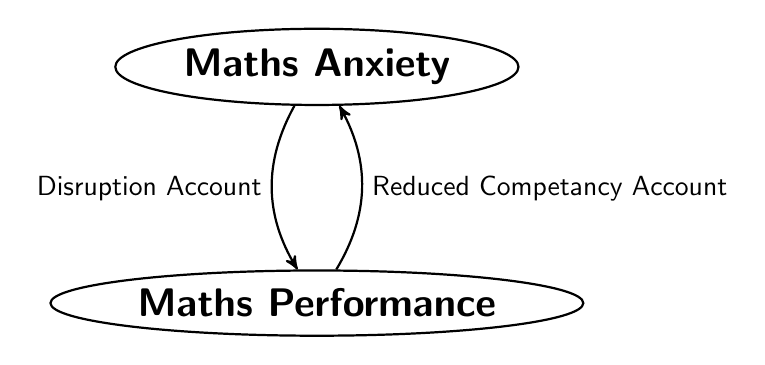
\begin{tikzpicture}[->,>=stealth',auto,node distance=3cm,thick,main node/.style={ellipse,draw,font=\sffamily\Large\bfseries}]
  	\node[main node] (a) {Maths Anxiety};
 	\node[main node] (b) [below of=a] {Maths Performance};

	\path	(a) edge[bend right] node [left] {Disruption Account} (b)
		(b) edge[bend right] node [right] {Reduced Competancy Account} (a);
\end{tikzpicture}
\end{document}
\caption{The Interpretation Account of Ramirez et al. (2018) for the maths anxiety-performance link showing how the Disruption Account and the Reduced Competency Account can be compatible.
\label{fig:ramirez}}
\end{center}
\end{figure}

First, a little more detail on the existing theories. The ``Disruption Account'', spearheaded by the work of Ashcraft et al., is centered around the concept of working memory \cite{Ashcraft2001, Ashcraft2007}. Specifically that anxiety about maths takes up students working memory, which prevents them from using that working memory to complete maths tasks and thereby impacts their performance. The ``Reduced Competency Account'' on the other hand proposes the opposite causality: that lower ability in maths leads to negative experiences associated to maths, which in turn cause maths anxiety to develop. There is also a significant body of work to support this hypothesis, including the milestone meta-analysis of \citeA{Hembree1990} and the longitudinal study of \citeA{Ma2004} which found that although past maths anxiety was correlated with future maths performance it was a small effect, while past maths performance had a strong effect on future maths anxiety.



\subsection*{Complexities in Finding Effective Interventions}

These theoretical views are of course broad oversimplifications of what is an incredibly complex and interconnected topic. They also imply very different approaches for intervention. The ``Reduced Competency Account'' would imply interventions to boost maths performance and hence allow students to experience success in math should also help to reduce maths anxiety. The results of  \citeA{Supekar2015} seem to support this hypothesis as when students are given an intensive 8-week tutoring program to boost their maths skills, this is associated to a reduction in maths anxiety. The earlier work by \citeA{Faust1996} further supports this by demonstrating an anxiety-complexity effect in which low and high maths anxiety groups performed similarly on low complexity problems, but in high complexity problems the high anxiety groups performance was impacted. On the other hand, \citeA{Jansen2013} showed that it is not neccessarily that simple, by showing that when students experience more success they attempt more problems and perform better. However their improved performance is almost completely predicted by the number of problems they attempted, not their experience of success, and their level of maths anxiety was not affected in a significant way which raises a lot of interesting but unanswered questions about this approach. 
	
On the other side of attempted interventions are those in line with the ``Disruption Account'', in which the maths anxiety itself is addressed in the hopes that will free up extra working memory and hence boost students performance.  \citeA{Park2014} demonstrate a direct and successful attempt at this in which they used expressive writing exercises to help guide students self-perceived narratives about their maths experiences and thereby reduce their maths anxiety. Notably the approach of \citeA{Park2014} is in line with successful treatments for clinical anxiety disorders (see \citeA{McNally2007, Becker2007,Foa2005}). Another approach that has shown success in this vein does not attempt to directly reduce the anxiety experienced, but rather reappraise it's symptoms \cite{Jamieson2016}. This is another technique from clinical psychology in which stress is reconceptualised as a coping tool, an evolutionary method for heightening performance in response to a challenge to be overcome, instead of a symptom of exposure to something to be feared and avoided. This change in the perspective of stress is also very much in line with the ``Interpretation Account'' of \citeA{Ramirez2018}.

The work of \citeA{Wang2015} showed the role that intrinsic motivation has mediating the relationship between maths anxiety and performance, and suggested the importance of a mindset centred on viewing the process of learning maths as one of ``productive struggle''. This reconceptualisation to a `productive struggle' model is supported by other literature as well, \citeA{Lin-Siegler2016} exposes students in a classroom to struggles experienced by famous scientists in order to help normalise the concept of productive struggle, and \citeA{Hiebert2007} discuss the importance of this same concept in a maths context.

One of the implications of the ``Interpretation Account'' is that if an intervention targets only one of these two possible links in the cycle (see \reffig{ramirez}), the cycle may re-establish itself after the intervention is over and negate any potential longterm effects. However there is only a very limited amount of research out there on such longterm effects, and several authors have discussed the need for further research into this \cite{Pellicioni2016,Chang2016}. My hypothesis is that a multi-faceted approach targetting both directions simultaneously could disrupt the cycle shown in \reffig{ramirez} and result in significant longterm effects.

\subsection*{Instruments for Measuring Maths Anxiety}

In order to track the effectiveness of these interventions, we will be collating assessment results as a measure of performance, but will also want to measure maths anxiety and maths affect/ self-concept. Significant work has been done over the years to develop psychometrics to measure maths anxiety, almost exclusively consisting of self-reporting surveys (with the exception of some more modern \gls{fmri} work, such as that of \citeA{Lyons2012}). We will use a recently developed scale: the \gls{mas-r} of \citeA{Bai2009}, which has been shown to be remarkably self consistent by incorporating both positive and negative affect items \cite{Bai2011}. It is short, easy to implement, and cheap in comparison to \gls{fmri} methods. In order to measure maths self-concept, \citeA{Jansen2013} modified the Perceived Competence Scale for Children of \citeA{Harter1982} to measure ``Math Competance''. The methodological process imployed by \citeA{Jansen2013} was quite rigorous and so we will use their instrument, or a minor modification thereof (we will do it in English), to measure maths self-concept.












\cleardoublepage
\chapter{Curriculum Mapping}
\label{chap:curriculum}

One of the important roles of university mathematics bridging courses (MathStart and MathTrack) is to fill the content knowledge gap for students who did not complete Mathematical Methods or Specialist Mathematics in highschool but wish to commence study at a university level in subjects that have required knowledge that in contained in these subjects. Although the \gls{ac} lays out the expected curriculum for senior highschool (years 11 and 12) mathematical methods and specialist mathematics, the exact content knowledge required varies dramatically depending on the university course. Beyond this, different states in Australia teach different curriculums in senior highschool, and some differ significantly from the \gls{ac}, some do not even use the terms ``Mathematical Methods'' and ``Specialist Mathematics'' at all. In South Australia we teach the \gls{sace}, and so the expected knowledge when entrying South Australian unviersities tends to be based on the \gls{sace} curriculum. A notable example of this was in 2018 when significant changes where made to the \gls{sace} senior mathematics curriculum, the University of Adelaide re-modelled the content in it's primary first year mathematics courses to better match the prior knowledge of the majority of new students coming from \gls{sace}. That said, it is still of interest to align the bridging courses with not only the \gls{sace} curriculum, but also with \gls{ac} as students enrolling in the bridging courses are not always intending to commence study in south australia. For example, students planning to commence study in a university interstate in the following year but currently living in south australia may be reccomended to the bridging courses by the university they are planning to go too.

This chapter will examine the alignment of the content of MathStart and MathTrack (the mathematics bridging courses offered at the university of adelaide) with the \gls{ac} and \gls{sace}. First, in \refsec{content}, some notation will be introduced and the content of each of the three curriculums will be reviewed:
\begin{itemize}
	\item The \gls{ac} senior mathematics subjects mathematical methods and specialist mathematics,
	\item The \gls{sace} curriculum stage 1 mathematics, stage 2 mathematical methods, and stage 2 specialist mathematics,
	\item The University of Adelaide's bridging courses: MathStart, and MathTrack.
\end{itemize}
Then, these will be mapped to each other in \refsec{mapping} (see \reffig{mapping}).
Throughout, discussion will be had around alignment and gaps between the content of these curriculums and courses, explanations and reasons for these discrepancies, and potential alternate approaches. 

Beyond that, this chapter will also briefly discuss the alignment of these bridging courses to first year university mathematics courses and bridging courses offered by other universities in Australia, and discuss the relationship between the gaps in alignment between the \gls{ac}/\gls{sace} and the bridging courses and the requirements of these first year university courses. 

%However, overall the focus is on the alignment of the bridging courses and \gls{ac}/ \gls{sace}, rather than their alignment to the first year university courses for one clear and important reason: not all students enrolling in these bridging courses are commencing these first year university courses, or may be doing so at a different university in which their first year content is different. Hence, it is most fair to attempt to align the content with the \gls{ac}/\gls{sace} as this is the content other students should be covering in highschool prior to enrolling in university in any case, and hence puts people at a fair standing with those students, and also being aligned with the \gls{ac} in particular is useful for guaranteeing a certain level of knowledge for enrollment in universities interstate. 

\section{Content}
\label{sec:content}

\subsection{Notation}

Each of the senior highschool curriculums, as well as the university bridging courses, being considered here is broken down into topics, with each topic containing a number of key concepts. In \refsec{mapping}, the alignment between these curriculums and bridging courses will be considered thoroughly at both a topic-level, and to the finer detail of particular key concepts. In order to abstract away some of the complexity of considering the topic-level alignment, and be able to present the topic-level alignment in a meaningful way abbreviated codes will be used to identify each topic. These abbreviated codes are presented in \reftab{notation} and will be used for the remainder of this chapter.

\begin{table}[h]
\caption{Abbreviated codes for topics within the \gls{ac} and \gls{sace} senior mathematics subjects: Mathematical Methods nd Specialist Mathematics, as well as the Unviersity of Adelaides bridging courses: MathStart and MathTrack. Square brackets ([]) are used to indicate numeric values that can vary. \label{tab:notation}}
\begin{tabular}{ll}
Code & Meaning \\ \hline
 & \\
MMu[\#1]t[\#2] & \gls{ac} Senior Mathematical Methods Unit [\#1], Topic [\#2] \\
MMu[\#1]t[\#2] & \gls{ac} Senior Specialist Mathematics Unit [\#1], Topic [\#2] \\
 & \\
S1M[\#] & \gls{sace} Stage 1 Mathematics, Topic [\#] \\
S2MM[\#] & \gls{sace} Stage 2 Mathematical Methods, Topic [\#] \\
S2SM[\#] & \gls{sace} Stage 2 Specialist Mathematics, Topic [\#] \\
 & \\
MS[\#] & Maths Start, Topic (Booklet) [\#] \\
MT[\#] & Maths Track, Topic (Booklet) [\#]
\end{tabular}
\end{table}

\subsection{Within-Topic Key Concepts}

Description of each topic in the \gls{ac} Mathematical Methods and Specialist Mathematics Topics, \gls{sace} stage 1 mathematics, stage 2 mathematical methods and stage 2 specialist mathematics, and the University of Adelaides MathStart and MathTrack programs. For brevity a code is used to identify each topic, see \reftab{notation} above, and then for each topic it's name is given in bold followed by a list of the key concepts covered in that topic. These are discussed at length below, and this table is intended to be used as reference material for that discussion.

Note: I generally omit ``interpretation'' concepts. For example in S1M2 on quadratics I include the key concepts around the Vertex Form and Factorised Form, but I do not include the interpretation fo roots and vertices, deducing these from the equation of a quadratic, or deducing the equation of a quadratic given these bits of information. These are more surrounding skills, which I think it is fair to assume should be taught along with the key concepts. To an experienced maths educator, the key concepts should be enough to deduce the required surrounding interpretative framework. 

Note: This is a huge table. I could maybe put it in an apprendix?

% Giant Table of Key Concepts
\documentclass[varwidth=144mm, 12pt]{standalone}

% Multi-page Tables
\usepackage{longtable}

% Math
\usepackage{amsfonts}
\usepackage{amsmath}

% CMU sans serif font.
\usepackage[T1]{fontenc}
\renewcommand*\familydefault{\sfdefault}

\begin{document}
\begin{longtable}{lp{.85\textwidth}}
Code & \textbf{Name} and Key Concepts \\ \hline
& \\ \endhead
%\multicolumn{2}{l}{\gls{ac} Senior Mathematical Methods} \\ 
MMu1t1 & \textbf{Functions and graphs}: Lines, Quadratics, Inverse Proportions, Polynomials, Relations, Translations and Dilations \\
MMu1t2 & \textbf{Trigonometric functions}: Unit Circle, Radians, SOH CAH TOA, Sine Rule, Exact Values, Amplitude/ Period/ Phase, Sum of Angles Identities \\
MMu1t3 & \textbf{Counting and probability}: Binomial Coefficients, Set Complement Intersection and Union, Probability, $P(A\cup{}B) = P(A) + P(B) - P(A\cap{}B)$, Conditional Probability, Independance \\
MMu2t1 & \textbf{Exponential functions}: Index Laws, Fractional Indices, Functions, Asymptotes, Graphs \\
MMu2t2 & \textbf{Arithmetic and geometric sequences and series}: Arithmetic and Geometric Sequences as Recurrence Relations, Limiting Behaviour, and Partial Sum Formulae, Growth and Decay \\
MMu2t3 & \textbf{Introduction to differential calculus} Average Rate of Change, First Principles, Leibniz Notation, Instantaneous Rate of Change, Slope of Tangent, Derivitive of Polynomials, Linearity of Differentiation, Optimisation, Anti-Derivitives, Interpret Position-Time Graphs \\
MMu3t1 & \textbf{Further differentiation and applications}: Define $e$ as $a$ s.t. $\lim_{h \to 0} \frac{a^h - 1}{h} = 1$, Derivitives of $e^x$ $\sin(x)$ and $\cos(x)$, Chain Product and Quotient Rules, Second Derivitives \\
MMu3t2 & \textbf{Integrals}: Integrate Polynomial Exponential and Trigonometric Functions, Linearity of Integration,  Determine Displacement given Velocity, Definite Integrals, Fundamental Theorem of Calculus, (signed) Area Under a Curve \\
MMu3t3 & \textbf{Discrete random variables}: Frequencies, General Properties, Expected Value, Variance, Standard Deviation, Bernoulli and Binomial Distribtions \\
MMu4t1 & \textbf{The logarithmic function}: Logs as Inverse of Exponentials, Log-Scales, Log Function Graphs, Natural Log, $\frac{d}{dx}\ln{x} = \frac{1}{x}$, $\int \frac{1}{x}dx = \ln{x} + c$ for $x > 0$ \\
MMu4t2 & \textbf{Continuous random variables and the normal distribution}: Probability Density Function, Cumulative Distribution Function, Probabilites Expected Value, Variance and Standard Deviation as Integrals, Linear Transformation of Random Variables, Normal Distribution using Technology \\
MMu4t3 & \textbf{Interval estimates for proportions} Simple Random Sampling, Bias, Sample Proportion, Normal Approximation to the Binomial Proportion, Wald Confidence Interval, Trade-Off Between Width and Level of Confidence \\
& \\
%\multicolumn{2}{l}{\gls{ac} Senior Specialist Mathematics} \\ 
SMu1t1 & \textbf{Combinatorics} Multiplication of Possibilities, Factorial Notation, Permutations with and without Repeated Objects, Union of Three Sets, Pigeon-Hole Principle, Combinations, Pascals Triangle \\
SMu1t2 & \textbf{Vectors in the plane}: Magnetude and Direction, Scalar Multiplication, Addition and Substraction as a Triangle, Vector Notation, $a\textbf{i} + b\textbf{j}$ Notation, Scalar Dot Product, Projection, Parallel and Perpendicular Vectors \\
SMu1t3 & \textbf{Geometry}: Notation for Implication ($\Rightarrow$) and Equivalence ($\Leftrightarrow$), Converse ($B \Rightarrow A$) Negation ($\neg A \Rightarrow \neg B$) and Contrapositive ($\neg B \Rightarrow \neg A$), Proof by Contradiction, $\forall$ and $\exists$ Notation, Counter-Examples, Circle Theorems, Quadrilateral Proofs in $\mathbb{R}^2$ \\
SMu2t1 & \textbf{Trigonometry}: Graph and Solve Trig Functions, Prove Various Trig Indentities, Reciprocal Trig Functions \\
SMu2t2 & \textbf{Matrices}: Notation, Addition and Scalar Multiplication of Matrices, Multiplicative Identity and Inverse, Determinant, Matrices as Transformations \\
SMu2t3 & \textbf{Real and complex numbers}: Rationality and Irrationality, Induction, $i = \sqrt{-1}$, Complex Numbers $a + bi$ and Arithmetic ($+$, $-$, $\times$, $\div$), Complex Conjugates, Complex Plane,  Complex Conjugate Roots of Polynomials \\
SMu3t1 & \textbf{Complex numbers}: Modulus and Argument, Arithmetic ($\times$, $\div$, and $z^n$) in Polar Form, Convert between Polar and Cartesian Form, De Moivre's Theorem, Roots of Complex Numbers, Factorising Polynomials \\
SMu3t2 & \textbf{Functions and sketching graphs}: Composition of Functions, One-to-One, Inverse Functions, Absolute Value Function, Rational Functions \\
SMu3t3 & \textbf{Vectors in three dimensions}: $a\textbf{i} + b\textbf{j} + c\textbf{k}$ Notation, Equation for Spheres, Parameterised Vector Equations, Equations of Lines, the Cross Product, Equation for a Plane, Systems of Linear Equation (Elimination Method) and Geometric Interpretation of Solutions, Kinematics via Differentiation of Vector Equations, Projectile and Circular Motion \\
SMu4t1 & \textbf{Integration and applications of integration} Substitution, $\int \frac{1}{x}dx = \ln{|x|} + c$ for $x \neq 0$, Inverse Trig Functions and their Derivitives, Integrate $\frac{\pm1}{\sqrt{a^2-x^2}}$ and $\frac{a}{a^2 + x^2}$, Partial Fractions, Integration by Parts, Volume of Solids of Revolution, Numerical Integration using Technology \\
SMu4t2 & \textbf{Rates of change and differential equations}: Implicit Differentiation, First-Order Seperable Differential Equations, The Logistic Equation, Kinematics (Rates of Change) \\
SMu4t3 & \textbf{Statistical inference}: Central Limit Theorem and the Resulting Confidence Interval for a Mean \\
& \\
%\multicolumn{2}{l}{\gls{sace} Stage 1 Mathematics} \\ 
S1M1 & \textbf{Functions and graphs}: Equations for a Line, Slope, y-intercept, Intersection of Lines, Reciprocal Function, Asymptotes, Functions vs Relations, Domain, Range, Function Notation \\
S1M2 & \textbf{Polynomials}: Quadratic Equations in Vertex and Factorised Forms, Quadratic Formula, Completing the Square, The Leading Coefficient and Degree of a Polynomials, Cubics, Quartics\\
S1M3 & \textbf{Trigonometry}: Pythagoras, SOH CAH TOA, Cosine Rule, Sine Rule, Unit Circle, Sine and Cosine Functions, Radians, Length of Arc, Area of Sector, Amplitude, Period, Phase, $\tan{x} = \frac{\sin{x}}{\cos{x}}$ \\
S1M4 & \textbf{Counting and statistics}: Factorial, Permutations, Multiplication Principle, Combinations, Discrete vs Continuous Random Variables, Mean, Median, Mode, Range, Interquartile Range, Standard Deviation, Normal Distribution, \\
S1M5 & \textbf{Growth and decay}: Index and Logarithm Laws, Exponential Functions and their Graphs \\
S1M6 & \textbf{Introduction to differential calculus}: Average Rate of Change, First Principles, Notation $f'(x) = \frac{df}{dx}$, $\frac{d}{dx}x^n = nx^{n-1}$, Linearity of Differentiation, Slope of Tangent, Increasing vs Decreasing, Local and Global Maxima and Minima, Stationary Points, Sign Diagram \\
S1M7 & \textbf{Arithmetic and geometric sequences and series}: \\
S1M8 & \textbf{Geometry}: \\
S1M9 & \textbf{Vectors in the plane}: \\
S1M10 & \textbf{Further Trigonometry}: \\
S1M11 & \textbf{Matrices}: \\
S1M12 & \textbf{Real and complex numbers}: \\
& \\
%\multicolumn{2}{l}{\gls{sace} Stage 2 Mathematical Methods} \\ 
S1MM1 & \textbf{Further differentiation and applications}: \\
S1MM2 & \textbf{Discrete random variables}: \\
S1MM3 & \textbf{Integral calculus}: \\
S1MM4 & \textbf{Logarithmic functions}: \\
S1MM5 & \textbf{Continuous random variables and the normal distribution}: \\
S1MM6 & \textbf{Sampling and confidence intervals}: \\
& \\
%\multicolumn{2}{l}{\gls{sace} Stage 2 Specialist Mathematics} \\ 
S1SM1 & \textbf{Mathematical induction}: \\
S1SM2 & \textbf{Complex numbers}: \\
S1SM3 & \textbf{Functions and sketching graphs}: \\
S1SM4 & \textbf{Vectors in three dimensions}: \\
S1SM5 & \textbf{Integration techniques and applications}: \\
S1SM6 & \textbf{Rates of change and differential equations}: \\
& \\
%\multicolumn{2}{l}{UofA MathStart} \\ 
MS1 & \textbf{Numbers \& Functions}: \\
MS2 & \textbf{Linear Functions}: \\
MS3 & \textbf{Quadratic Functions}: \\
MS4 & \textbf{Rational Functions}: \\
MS5 & \textbf{Trigonometry I}: \\
MS6 & \textbf{Trigonometry II}: \\
MS7 & \textbf{Exponential Functions}: \\
MS8 & \textbf{Logarithms}: \\
& \\
%\multicolumn{2}{l}{UofA MathTrack} \\ 
MT1 & \textbf{Polynomials}: \\
MT2 & \textbf{Matrices}: \\
MT3 & \textbf{Vectors and Applications}: \\
MT4 & \textbf{Systems of Linear Equations}: \\
MT6 & \textbf{Differentiation}: \\
MT7 & \textbf{Applications of Differentiation}: \\
MT8 & \textbf{Exponential and Logarithm Functions}: \\
MT9 & \textbf{Integration}: \\
\end{longtable}
\end{document}


\subsection{\gls{ac} Mathematical Methods and Specialist Mathematics}

 \gls{ac} has four levels of mathmatics, including also essential and general mathematics. Mathematical Methods and Specialist Mathematics are the two highest level mathematics, intended (partly) for preparation to university entry.

\subsection{\gls{sace} Stage 1 Mathematics, Stage 2 Mathematical Methods and Specialist Mathematics}

Cumulative Distribution Function not mentioned


\subsection{MathStart and MathTrack}

Note the missing topic 5 in MathTrack, this used to be part of the course some time ago but is now ommitted.










\section{Curriculum Mapping}
\label{sec:mapping}

\reffig{mapping} shows the topic-level alignment between the \gls{ac} (senior mathematical methods and specialist mathematics), \gls{sace} (mathematical methods and specialist mathematics), MathStart and MathTrack. Although sub-topic alignment within these topic alignments is not always perfect, it is fairly strong in each case but individual cases will be discussed in more detail below.

\begin{figure}[p]
\begin{center}
% TiKz
\documentclass[tikz, 12pt]{standalone}
\usetikzlibrary{positioning}
\usetikzlibrary{shapes}

% Math
\usepackage{amsfonts}
\usepackage{amsmath}

% CMU sans serif font.
\usepackage[T1]{fontenc}
\renewcommand*\familydefault{\sfdefault}

\begin{document}
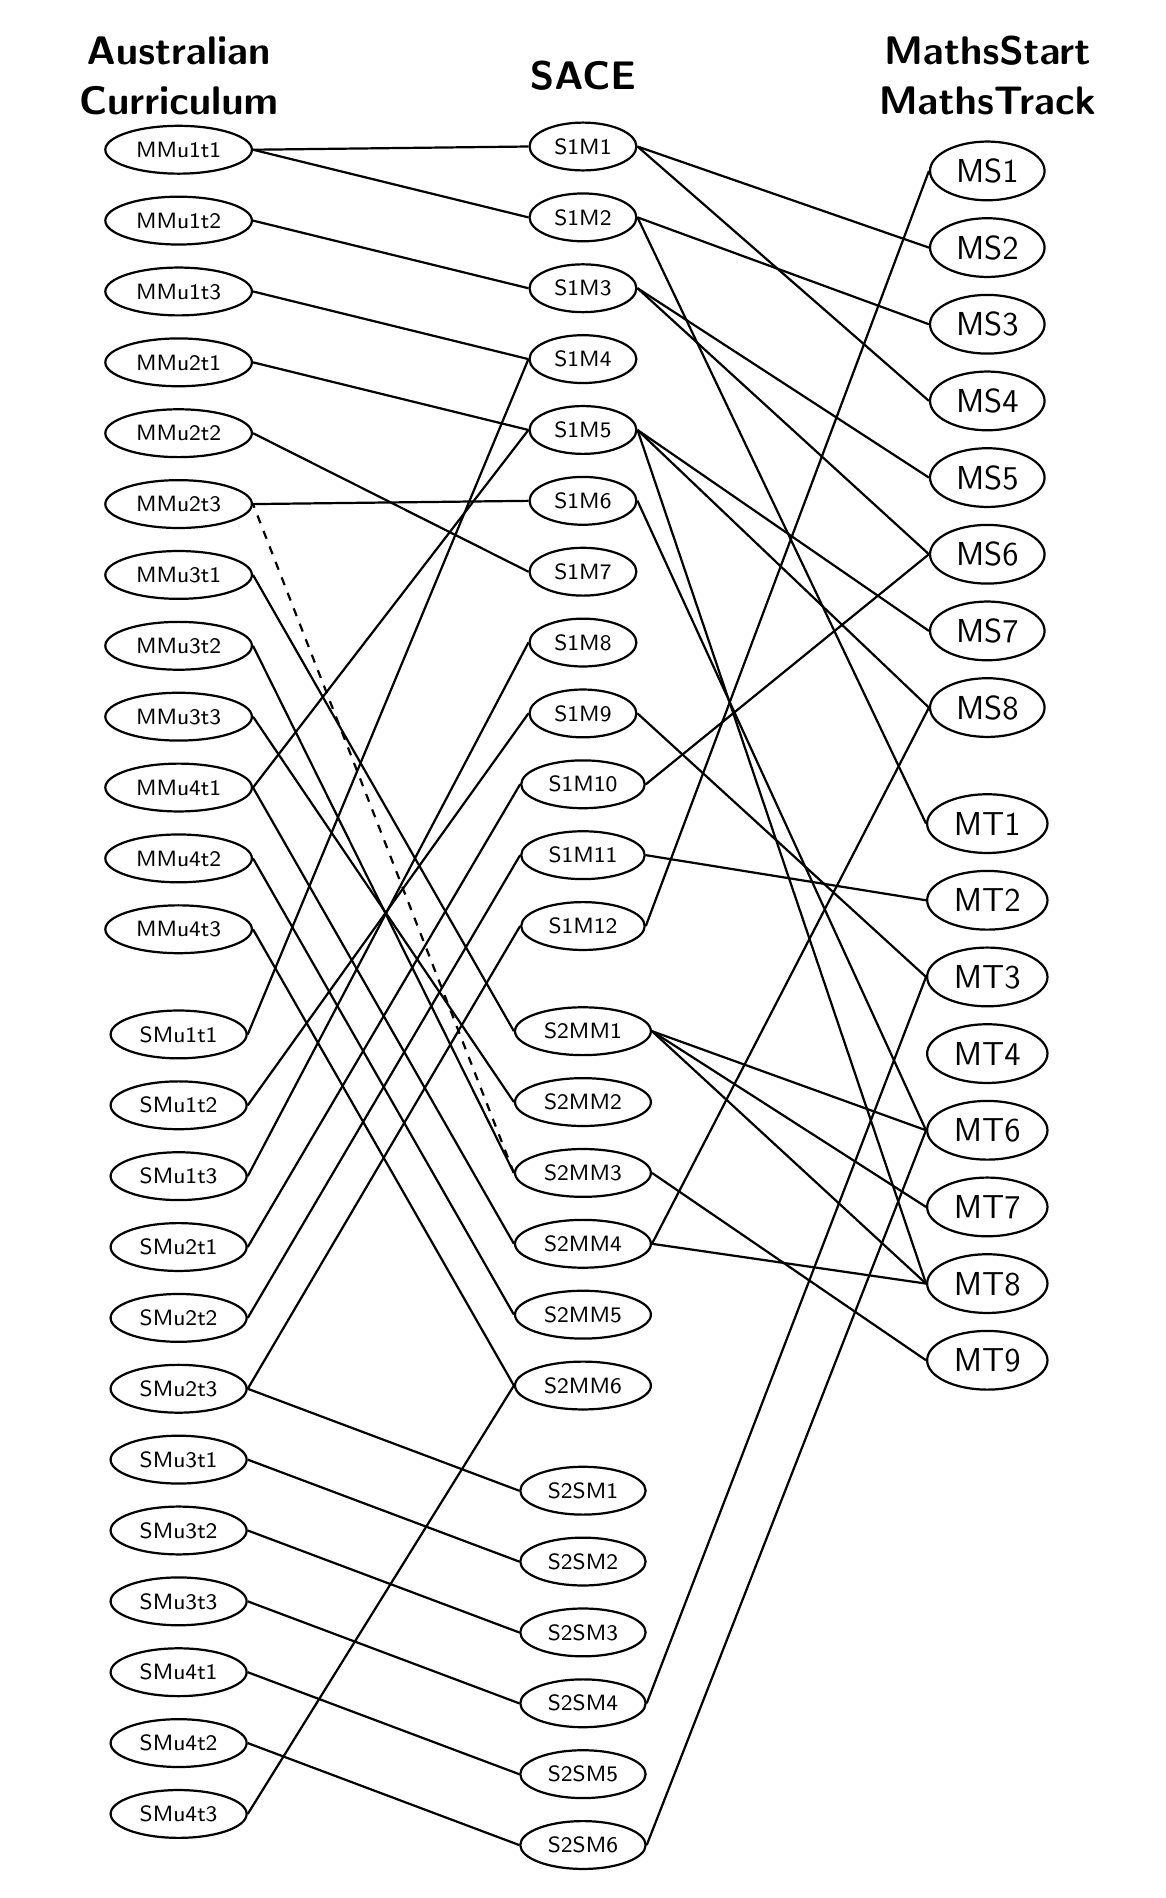
\begin{tikzpicture}[node distance=0.9cm,thick,topic node/.style={ellipse,draw,font=\footnotesize},unit node/.style={ellipse,draw,font=\large}]

	% MathsStart
	\node[font=\Large\bfseries, text width = 3.6cm, align=center] (ms) {MathsStart MathsTrack};
  	\node[unit node] (ms1) [below=0.2cm of ms] {MS1};
  	\node[unit node] (ms2) [below=0.2cm of ms1] {MS2};
  	\node[unit node] (ms3) [below=0.2cm of ms2] {MS3};
  	\node[unit node] (ms4) [below=0.2cm of ms3] {MS4};
  	\node[unit node] (ms5) [below=0.2cm of ms4] {MS5};
  	\node[unit node] (ms6) [below=0.2cm of ms5] {MS6};
  	\node[unit node] (ms7) [below=0.2cm of ms6] {MS7};
  	\node[unit node] (ms8) [below=0.2cm of ms7] {MS8};
%  	\node[unit node] (ms1) [below=0.2cm of ms] {Functions};
%  	\node[unit node] (ms2) [below=0.2cm of ms1] {Linear};
%  	\node[unit node] (ms3) [below=0.2cm of ms2] {Quadratic};
%  	\node[unit node] (ms4) [below=0.2cm of ms3] {Rational};
%  	\node[unit node] (ms5) [below=0.2cm of ms4] {Trigonometry I};
%  	\node[unit node] (ms6) [below=0.2cm of ms5] {Trigonometry II};
%  	\node[unit node] (ms7) [below=0.2cm of ms6] {Exponential};
%  	\node[unit node] (ms8) [below=0.2cm of ms7] {Logarithm};

	% MathsTrack
  	\node[unit node] (mt1) [below=0.7cm of ms8] {MT1};
  	\node[unit node] (mt2) [below=0.2cm of mt1] {MT2};
  	\node[unit node] (mt3) [below=0.2cm of mt2] {MT3};
  	\node[unit node] (mt4) [below=0.2cm of mt3] {MT4};
  	\node[unit node] (mt6) [below=0.2cm of mt4] {MT6};
  	\node[unit node] (mt7) [below=0.2cm of mt6] {MT7};
  	\node[unit node] (mt8) [below=0.2cm of mt7] {MT8};
  	\node[unit node] (mt9) [below=0.2cm of mt8] {MT9};
%  	\node[unit node] (mt1) [below=0.8cm of ms8] {Polynomials};
%  	\node[unit node] (mt2) [below=0.2cm of mt1] {Matrices};
%  	\node[unit node] (mt3) [below=0.2cm of mt2] {Vectors};
%  	\node[unit node] (mt4) [below=0.2cm of mt3] {Systems of Eqns};
%  	\node[unit node] (mt6) [below=0.2cm of mt4] {Differentiation};
%  	\node[unit node] (mt7) [below=0.2cm of mt6] {Differentiation Apps};
%  	\node[unit node] (mt8) [below=0.2cm of mt7] {Exp and Log};
%  	\node[unit node] (mt9) [below=0.2cm of mt8] {Integration};
  	
	% SACE
	\node[font=\Large\bfseries] (sace) [left=2.4cm of ms] {SACE};
  	\node[topic node] (ss1m1) [below of=sace] {S1M1};
  	\node[topic node] (ss1m2) [below of=ss1m1] {S1M2};
  	\node[topic node] (ss1m3) [below of=ss1m2] {S1M3};
  	\node[topic node] (ss1m4) [below of=ss1m3] {S1M4};
  	\node[topic node] (ss1m5) [below of=ss1m4] {S1M5};
  	\node[topic node] (ss1m6) [below of=ss1m5] {S1M6};
  	\node[topic node] (ss1m7) [below of=ss1m6] {S1M7};
  	\node[topic node] (ss1m8) [below of=ss1m7] {S1M8};
  	\node[topic node] (ss1m9) [below of=ss1m8] {S1M9};
  	\node[topic node] (ss1m10) [below of=ss1m9] {S1M10};
  	\node[topic node] (ss1m11) [below of=ss1m10] {S1M11};
  	\node[topic node] (ss1m12) [below of=ss1m11] {S1M12};
%  	\node[topic node] (ss1m1) [below of=sace] {Functions I};
%  	\node[topic node] (ss1m2) [below of=ss1m1] {Polynomials};
%  	\node[topic node] (ss1m3) [below of=ss1m2] {Trigonometry I};
%  	\node[topic node] (ss1m4) [below of=ss1m3] {Combinatorics};
%  	\node[topic node] (ss1m5) [below of=ss1m4] {Exponentials};
%  	\node[topic node] (ss1m6) [below of=ss1m5] {Differentiation I};
%  	\node[topic node] (ss1m7) [below of=ss1m6] {Sequences};
%  	\node[topic node] (ss1m8) [below of=ss1m7] {Circle Theorems};
%  	\node[topic node] (ss1m9) [below of=ss1m8] {Vectors ($\mathbb{R}^2$)};
%  	\node[topic node] (ss1m10) [below of=ss1m9] {Trigonometry II};
%  	\node[topic node] (ss1m11) [below of=ss1m10] {Matrices};
%  	\node[topic node] (ss1m12) [below of=ss1m11] {Complex ($\mathbb{C}$) I};
  	
  	\node[topic node] (ss2mm1) [below=0.7cm of ss1m12] {S2MM1};
  	\node[topic node] (ss2mm2) [below of=ss2mm1] {S2MM2};
  	\node[topic node] (ss2mm3) [below of=ss2mm2] {S2MM3};
  	\node[topic node] (ss2mm4) [below of=ss2mm3] {S2MM4};
  	\node[topic node] (ss2mm5) [below of=ss2mm4] {S2MM5};
  	\node[topic node] (ss2mm6) [below of=ss2mm5] {S2MM6};
%  	\node[topic node] (ss2mm1) [below=1cm of ss1m12] {Differentiation II};
%  	\node[topic node] (ss2mm2) [below of=ss2mm1] {Discrete RV};
%  	\node[topic node] (ss2mm3) [below of=ss2mm2] {Integration I};
%  	\node[topic node] (ss2mm4) [below of=ss2mm3] {Logarithms};
%  	\node[topic node] (ss2mm5) [below of=ss2mm4] {Continuous RV};
%  	\node[topic node] (ss2mm6) [below of=ss2mm5] {Sampling};
  	
  	\node[topic node] (ss2sm1) [below=0.7cm of ss2mm6] {S2SM1};
  	\node[topic node] (ss2sm2) [below of=ss2sm1] {S2SM2};
  	\node[topic node] (ss2sm3) [below of=ss2sm2] {S2SM3};
  	\node[topic node] (ss2sm4) [below of=ss2sm3] {S2SM4};
  	\node[topic node] (ss2sm5) [below of=ss2sm4] {S2SM5};
  	\node[topic node] (ss2sm6) [below of=ss2sm5] {S2SM6};  	
%  	\node[topic node] (ss2sm1) [below=1cm of ss2mm6] {Induction};
%  	\node[topic node] (ss2sm2) [below of=ss2sm1] {Complex ($\mathbb{C}$) II};
%  	\node[topic node] (ss2sm3) [below of=ss2sm2] {Functions II};
%  	\node[topic node] (ss2sm4) [below of=ss2sm3] {Vectors ($\mathbb{R}^3$)};
%  	\node[topic node] (ss2sm5) [below of=ss2sm4] {Integration II};
%  	\node[topic node] (ss2sm6) [below of=ss2sm5] {DEs};  	
  	
	% Australian Curriculum
	\node[font=\Large\bfseries, text width = 3.6cm, align=center] (ac) [left=2.4cm of sace] {Australian Curriculum};
  	\node[topic node] (acmmmu1t1) [below=0cm of ac] {MMu1t1};
  	\node[topic node] (acmmmu1t2) [below of=acmmmu1t1] {MMu1t2};
  	\node[topic node] (acmmmu1t3) [below of=acmmmu1t2] {MMu1t3};
  	\node[topic node] (acmmmu2t1) [below of=acmmmu1t3] {MMu2t1};
  	\node[topic node] (acmmmu2t2) [below of=acmmmu2t1] {MMu2t2};
  	\node[topic node] (acmmmu2t3) [below of=acmmmu2t2] {MMu2t3};
  	\node[topic node] (acmmmu3t1) [below of=acmmmu2t3] {MMu3t1};
  	\node[topic node] (acmmmu3t2) [below of=acmmmu3t1] {MMu3t2};
  	\node[topic node] (acmmmu3t3) [below of=acmmmu3t2] {MMu3t3};
  	\node[topic node] (acmmmu4t1) [below of=acmmmu3t3] {MMu4t1};
  	\node[topic node] (acmmmu4t2) [below of=acmmmu4t1] {MMu4t2};
  	\node[topic node] (acmmmu4t3) [below of=acmmmu4t2] {MMu4t3};
  	
  	\node[topic node] (acmsmu1t1) [below=0.7cm of acmmmu4t3] {SMu1t1};
  	\node[topic node] (acmsmu1t2) [below of=acmsmu1t1] {SMu1t2};
  	\node[topic node] (acmsmu1t3) [below of=acmsmu1t2] {SMu1t3};
  	\node[topic node] (acmsmu2t1) [below of=acmsmu1t3] {SMu2t1};
  	\node[topic node] (acmsmu2t2) [below of=acmsmu2t1] {SMu2t2};
  	\node[topic node] (acmsmu2t3) [below of=acmsmu2t2] {SMu2t3};
  	\node[topic node] (acmsmu3t1) [below of=acmsmu2t3] {SMu3t1};
  	\node[topic node] (acmsmu3t2) [below of=acmsmu3t1] {SMu3t2};
  	\node[topic node] (acmsmu3t3) [below of=acmsmu3t2] {SMu3t3};
  	\node[topic node] (acmsmu4t1) [below of=acmsmu3t3] {SMu4t1};
  	\node[topic node] (acmsmu4t2) [below of=acmsmu4t1] {SMu4t2};
  	\node[topic node] (acmsmu4t3) [below of=acmsmu4t2] {SMu4t3};

	% Australian Curriculum -- SACE links
	\draw (ss1m1.west) -- (acmmmu1t1.east);
	\draw (ss1m2.west) -- (acmmmu1t1.east);
	\draw (ss1m3.west) -- (acmmmu1t2.east);
	\draw (ss1m4.west) -- (acmmmu1t3.east);
	\draw (ss1m4.west) -- (acmsmu1t1.east);
	\draw (ss1m5.west) -- (acmmmu2t1.east);
	\draw (ss1m5.west) -- (acmmmu4t1.east);
	\draw (ss1m6.west) -- (acmmmu2t3.east);
	\draw (ss1m7.west) -- (acmmmu2t2.east);
	\draw (ss1m8.west) -- (acmsmu1t3.east);
	\draw (ss1m9.west) -- (acmsmu1t2.east);
	\draw (ss1m10.west) -- (acmsmu2t1.east);
	\draw (ss1m11.west) -- (acmsmu2t2.east);
	\draw (ss1m12.west) -- (acmsmu2t3.east);
		
	\draw (ss2mm1.west) -- (acmmmu3t1.east);
	\draw (ss2mm2.west) -- (acmmmu3t3.east);
	\draw (ss2mm3.west) -- (acmmmu3t2.east);
	\draw[dashed] (ss2mm3.west) -- (acmmmu2t3.east);
	\draw (ss2mm4.west) -- (acmmmu4t1.east);
	\draw (ss2mm5.west) -- (acmmmu4t2.east);
	\draw (ss2mm6.west) -- (acmmmu4t3.east);
	\draw (ss2mm6.west) -- (acmsmu4t3.east);

	\draw (ss2sm1.west) -- (acmsmu2t3.east);
	\draw (ss2sm2.west) -- (acmsmu3t1.east);
	\draw (ss2sm3.west) -- (acmsmu3t2.east);
	\draw (ss2sm4.west) -- (acmsmu3t3.east);
	\draw (ss2sm5.west) -- (acmsmu4t1.east);
	\draw (ss2sm6.west) -- (acmsmu4t2.east);

	% MathsTrack to SACE links
	\draw (mt1.west) -- (ss1m2.east);
	\draw (mt2.west) -- (ss1m11.east);
	\draw (mt3.west) -- (ss1m9.east);
	\draw (mt3.west) -- (ss2sm4.east);
	\draw (mt6.west) -- (ss1m6.east);
	\draw (mt6.west) -- (ss2mm1.east);
	\draw (mt6.west) -- (ss2sm6.east);
	\draw (mt7.west) -- (ss2mm1.east);
	\draw (mt8.west) -- (ss1m5.east);
	\draw (mt8.west) -- (ss2mm1.east);
	\draw (mt8.west) -- (ss2mm4.east);
	\draw (mt9.west) -- (ss2mm3.east);

	% MathsStart to SACE links
	\draw (ms1.west) -- (ss1m12.east);
	\draw (ms2.west) -- (ss1m1.east);
	\draw (ms3.west) -- (ss1m2.east);
	\draw (ms4.west) -- (ss1m1.east);
	\draw (ms5.west) -- (ss1m3.east);
	\draw (ms6.west) -- (ss1m3.east);
	\draw (ms6.west) -- (ss1m10.east);
	\draw (ms7.west) -- (ss1m5.east);
	\draw (ms8.west) -- (ss1m5.east);
	\draw (ms8.west) -- (ss2mm4.east);
	

  	
\end{tikzpicture}
\end{document}
\caption{Curriculum Mapping
\label{fig:mapping}}
\end{center}
\end{figure}









\cleardoublepage
\chapter{Moving Forward: Improvements} 
\label{chap:recommendations}

\lipsum[1-2]

\cleardoublepage
\chapter*{Conclusions and Reccomendations}
\addcontentsline{toc}{chapter}{Conclusions and Reccomendations}

With respect to the bridging courses run through the university of adelaide's maths learning centre: MathsStart and MathsTrack,
\begin{itemize}
	\item The self-paced and feedback focused approach to assessment is certainly the highlight of the programs, should be continued, encouraged, potentially further resourced, expanded, and reccomended to other bridging course facilitators.
	\item The role of bridging courses as what is often student's first experience at university implies that potentially students wellbeing and retention could be improved by structuring the programs to provide more opportunities for students to meet each other and work together: either in the maths learning center drop-in area, or a seperate area, but potentially assigning a certain time on a certain day perhaps weekly or fortnightly during which students are encouraged to come and work together, could allow them to make freinds, build social networks, and better aclimitise them to the university environment in order to better prepare them for success in their studies.
	\item The smallest but perhaps easiest to implement improvement could be to better align the course content with curriculum, both the highschool curriculum (\gls{ac}/ \gls{sace}) in the case of students doing the bridging course to then comence study interstate or overseas, or with specific first year entry level courses, to better match the potential gaps in knowledge students may encounter.
\end{itemize}

% Bibliography/ References
\glsresetall
\bibliographystyle{apacite}
\bibliography{citations} 

\end{document}


